% This is LLNCS.DEM the demonstration file of
% the LaTeX macro package from Springer-Verlag
% for Lecture Notes in Computer Science,
% version 2.4 for LaTeX2e as of 16. April 2010
%
\documentclass{llncs}
%\documentclass[runningheads]{llncs}

% *** GRAPHICS RELATED PACKAGES ***
\usepackage{graphicx}
% declare the path(s) where your graphic files are
\graphicspath{{./Figs/}}
% and their extensions so you won't have to specify these with
% every instance of \includegraphics
\DeclareGraphicsExtensions{.pdf,.jpeg,.png}

%% ------ Packages added by pete ------ %%
%% ------ packages for authors format  ------ %%
\usepackage[misc]{ifsym}
\usepackage{bbding}
\usepackage{url}

\urldef{\mailsa}\path|{yuwenping}@mail.nankai.edu.cn|
\urldef{\mailsb}\path|{zhangjz, xujd, xuyw}@nankai.edu.cn|
%% ------ packages for authors format  ------ %%

%% ------ packages for subfigures  ------ %%
\usepackage[caption=false,font=footnotesize]{subfig}
%\usepackage{caption}
%\usepackage[justification=centering]{caption}

%% ------ packages for algorithm expressed with the pseudocode  ------ %%
\usepackage{algorithm}
%\usepackage{algorithmic}
\usepackage{algcompatible}

%% ------ packages for list  ------ %%
%\usepackage{enumitem}% http://ctan.org/pkg/enumitem


%% ------ typesetting with little spacing ------ %%
%%% Save the class definition of \subparagraph
%\let\llncssubparagraph\subparagraph
%%% Provide a definition to \subparagraph to keep titlesec happy
%\let\subparagraph\paragraph
%%% Load titlesec
%\usepackage[compact]{titlesec}
%%% Revert \subparagraph to the llncs definition
%\let\subparagraph\llncssubparagraph

\begin{document}

%%
%\mainmatter              % start of the contributions
%
\title{Motion Trajectory Sequence-Based Map Matching Assisted Indoor Autonomous Mobile Robot Positioning}
%J
\titlerunning{MTTSMatch}  % abbreviated title (for running head)
%                                     also used for the TOC unless
%                                     \toctitle is used
%
%%\author{Wenping Yu\inst{1}}

\author{Wenping Yu$^1$ \and Jianzhong Zhang$^2$ $^($\Envelope$^)$ \and Jingdong Xu$^2$ \and Yuwei Xu$^2$}
%
\authorrunning{Wenping Yu et al.} % abbreviated author list (for running head)
%
%%%% list of authors for the TOC (use if author list has to be modified)
\tocauthor{Wenping Yu}
%
\institute{College of Computer and Control Engineering, Nankai University, Tianjin, China\\
$^1$\mailsa\\
$^2$\mailsb\\}


\maketitle              % typeset the title of the contribution

\begin{abstract}

Position information is one of basic elements for context awareness of autonomous mobile robots. This paper studies the positioning algorithm of autonomous mobile robots suitable for search and rescue in dark building corridors and underground mine tunnels when an emergency occurs, and proposes a novel map matching aided positioning algorithm based on Hidden Markov Model. This algorithm does not rely on a camera, and only uses the inertial sensors installed in mobile robot and the indoor map to realize the fusion of dead reckoning and map matching. Firstly, it detects the position-related motion postures during the motion process, and then the motion trajectory is divided into a sub-trajectory sequence. By matching the sub-trajectory sequence with the indoor map, the proposed algorithm achieves tracking and positioning of mobile robots. In order to verify the effectiveness of our proposed algorithm, this paper adopts four-wheel differentially driven robot to conduct experimental analysis in an actual indoor scenario. The experimental results show that compared with the traditional dead reckoning technology, this algorithm can distinctly reduce the average positioning error of mobile robot, and it is robust to heading angle and acceleration noises within a certain error range.

\keywords{Mobile Robot \and Indoor Positioning \and Hidden Markov Model \and Posture Pattern Detection.}
\end{abstract}
%
\section{Introduction}
%
With the advancement of artificial intelligence, network and sensor technologies, the research and application of autonomous mobile robots have made remarkable progress in recent years. Indoor autonomous mobile robots are increasingly integrated into people's daily lives \cite{Garcia2007The}. Autonomous mobile robots can be extensively used not only in modern intelligent warehouses, home services and many other aspects, but also in corridors of complex buildings, tunnels of subway and underground mines when accidents occur. Therefore, the research of indoor autonomous mobile robot technology has gradually become a hot topic, and many domestic research institutes such as Tsinghua University, Harbin Institute of Technology, Nankai University and South China University of Technology are committed to the research and development of indoor autonomous mobile robots \cite{Wu2005Robust,Wu2015A,Yang2015An,yuan2009sprb,yuningbo2017RGBDbae}. The autonomous positioning of the mobile robot is a process in which the robot autonomously determines its position in the working environment, and is one of the most basic problems in improving the autonomous capabilities of the mobile robot.

In terms of outdoor positioning, the Global Positioning System (GPS) has become a widely used positioning technology for mobile robots. However, in terms of indoor positioning, due to the blocking and interference of GPS signals by the external walls of buildings and indoor complex electromagnetic environment, there is no universal solution to the positioning problem of indoor mobile robots \cite{Bachrach2011RANGE,bao2013indoor}. Currently, researchers have proposed a variety of positioning methods for indoor autonomous mobile robots, including navigation beacon-based positioning \cite{Tang2014multiary}, computer vision-based positioning \cite{lu2015visual,gao2017unsupervised}, dead reckoning positioning \cite{kim2015dead}, map matching positioning \cite{grisetti2007improved,cheng2015topological} and simultaneous localization and mapping (SLAM) \cite{de2014feature,havangi2014square}, and so on. Positioning techniques based on navigation beacons rely on a series of deployed feature signals to provide stable and accurate location information, but require high deployment and maintenance costs. Dead reckoning technique uses inertial sensors or encoders to provide relatively accurate positions over short distances, but exists cumulative error that gradually increases as the distance travels, and the robot's starting point needs to be known in advance. Map matching positioning uses known indoor maps to construct topological maps, feature maps, and other abstract maps, and then the position of the mobile robot is obtained by matching the robot motion trajectory with the indoor maps. The real-time performance of map matching is relatively poor according to its realization principle. The SLAM technology has unique advantages in the face of unknown environments and can provide indoor floor plans or 3D maps while providing positioning \cite{richter2018bayesian}. However, this method requires mobile robots equipped with more complex sensor devices, such as infrared, ultrasonic radar and RGB-D vision systems. Therefore, it has higher implementation cost.

Corridors of buildings, subway station tunnels and underground mines often have complex passageways, similar to “mazes”. In the event of an accident such as a fire, the power supply is damaged, the communication infrastructure become unusable and smoke and dust cause the lack of indoor lighting, and so on. All these situations pose challenges for the positioning of indoor autonomous mobile robots. Due to limitations in working environment or deployment conditions, it is difficult to establish visual or wireless navigation beacons in advance. Therefore, positioning technology based on navigation beacons is not suitable; the influence of high temperature and smoke on the indoor environment makes it difficult for cameras to provide image information, visual positioning technology fails; the timeliness of SLAM technology can not meet the urgent need for time factors in the above scenarios. In response to these problems, this paper introduces a hidden Markov model (HMM) based map matching algorithm that does not rely on a camera, only uses inertial sensors (accelerometers, gyroscopes, and magnetometers) installed in autonomous mobile robots and known indoor maps to effectively track and position mobile robots.

%In summary, this paper's mainly contributions are as follows:
%\vspace{-10pt}
%\begin{itemize}
%	\setlength{\parskip}{0pt} 
%	\setlength{\itemsep}{0pt plus 1pt}
%	\renewcommand{\labelitemi}{$\vcenter{\hbox{\tiny$\bullet$}}$}
%	\item we present the architecture of AiFiMatch: a map matching algorithm based on activity detection and crowd-sourced Wi-Fi.
%	\item we present the architecture of AiFiMatch: a map matching algorithm based on activity detection and crowd-sourced Wi-Fi.
%\end{itemize}
%\vspace{-8pt}

%In summary, this paper's mainly contributions are as follows:
%\begin{itemize}[noitemsep,topsep=0pt]
%	\renewcommand{\labelitemi}{$\vcenter{\hbox{\tiny$\bullet$}}$}
%	\item we present the architecture of AiFiMatch: a map matching algorithm based on activity detection and crowd-sourced Wi-Fi.
%	\item we present the architecture of AiFiMatch: a map matching algorithm based on activity detection and crowd-sourced Wi-Fi.
%\end{itemize}

The remainder of this paper is organized as follows: Section II introduces the robot motion model, the overview of proposed algorithm and its preprocessing components. Then, we detail the proposed HMM-based map matching algorithm in Section III. Section IV shows the experimental results and analysis. Finally, Section V concludes this paper.

\section{Robot Motion Model and Positioning Method}

In the field of indoor autonomous mobile robot positioning, dead reckoning technology and map matching technology have a good complementarity. This paper proposes a map matching-assisted positioning method based on motion trajectory sequence of mobile robot to realize the fusion of the above two technologies. The positioning algorithm uses stairs and corridor corners in the indoor environment as virtual landmarks. When the mobile robot passes through these landmarks, the inertial sensor data will show a specific pattern. Therefore, in this paper, the above landmarks are called posture-related positions. When the robot's movement distance is short, the dead reckoning technology can give the real-time position of the robot. When the robot's movement distance is long, the robot's motion trajectory can be divided into multiple sub-trajectories according to the landmarks, consecutive sub-trajectories form sub-trajectory sequence. With the help of HMM model, the above sub-trajectory sequence can be matched to the corresponding road in the indoor map, and then the position estimation of the mobile robot is given. Further, when the robot's motion trajectory is long enough, the absolute position of the mobile robot can still be estimated even without knowing the robot's starting point.

This section firstly introduces the simplified motion model of the four-wheel differential-driven autonomous mobile robot used in subsequent experiments, and derives the dead reckoning algorithm based on the motion model. Then, the overall architecture of the fusion positioning algorithm presented in this paper is introduced. Lastly, the indoor floor plan abstraction module and the mobile robot motion posture detection module are explained. The motion trajectory matching technology based on Hidden Markov Models is the core module of the positioning algorithm, which will be discussed in detail in the next section.

\subsection{Robot Motion Model and Its Dead Reckoning Algorithm}

In this paper, a four-wheel differential-driven mobile robot is used to study the positioning problem of autonomous mobile robots in indoor environment. The driving motor is a direct-current (DC) motor. The two driving motors on one side are connected in reverse parallel and use the \emph{L298N} motor driving module to control the DC motor, and the mobile robot adopts the Raspberry Pi \emph{B.V1.2} as the main control chip. According to the driving mode of the mobile robot, the motion models of the two wheels on each side of the wheeled robot are the same. Therefore, the motion model of the mobile robot can be simplified to a left and right two-wheel differential driving mode. Fig. \ref{fig-model-dr} (a) shows the simplified motion model of the mobile robot, where $(x, y)$ is the position coordinate of the mobile robot in the global coordinate system, $\Theta$ is the angle between heading direction of the mobile robot and the true north direction.

\begin{figure}[!htbp]
	\centering
	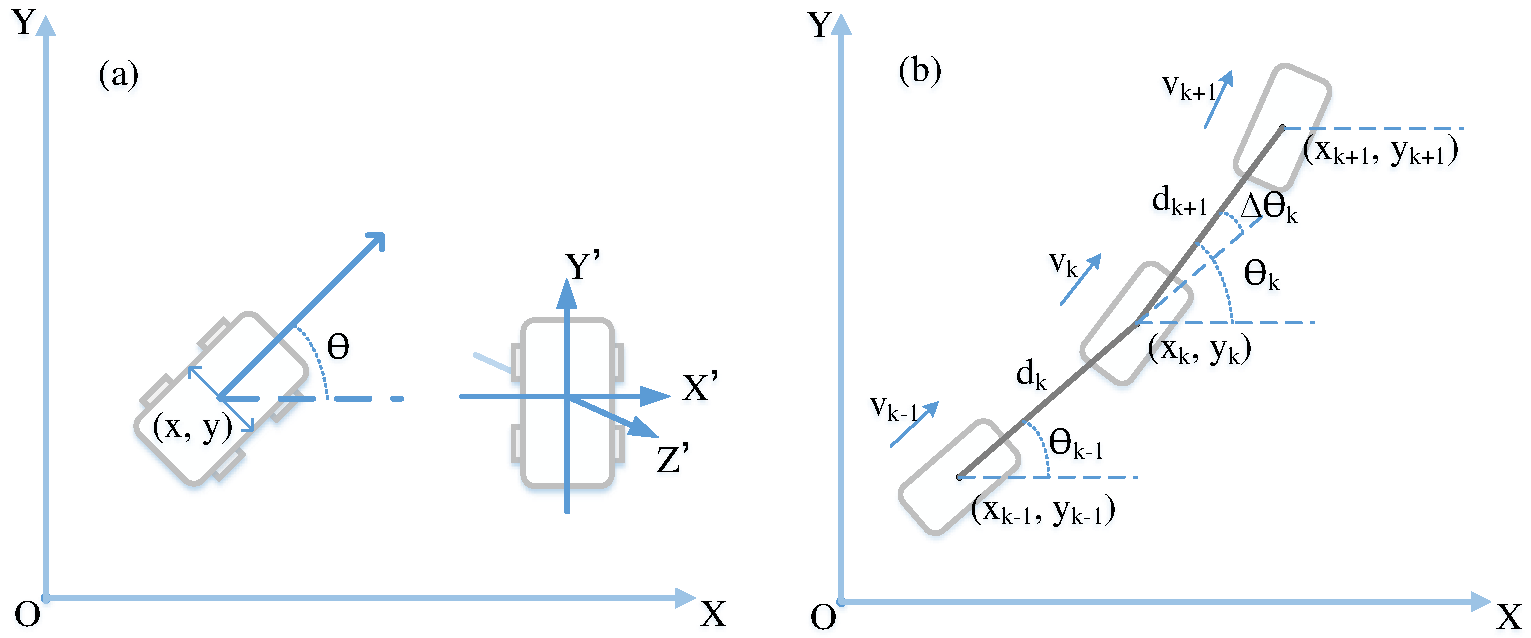
\includegraphics[width=4.7in]{RobotMatch-MotionModel}
	\caption{Simplified motion model and its dead reckoning principle for four-wheel differentially driven robot. (a) Motion model and self coordinate system. (b) Dead reckoning in the global coordinate system.}
	\label{fig-model-dr}
\end{figure}

Dead reckoning algorithm is widely used in the positioning of indoor autonomous mobile robots, and it is particularly suitable for short-range positioning. The autonomous mobile robot used in this paper has built-in digital compass, three-axis accelerometer and gyroscope. The digital compass gives the initial attitude of the mobile robot. The accelerometer and the gyroscope can measure the movement acceleration and rotation angular velocity of the mobile robot. The distance and heading direction change of the mobile robot can be obtained by integration, then we can derive the latest position and posture of the mobile robot.

In order to determine the position and posture of the mobile robot in the plane, we establish the global coordinate system $OXY$. Assuming that the starting point $(x_0, y_0)$ is the origin of the coordinates and the starting attitude is the positive direction of the $X$-axis, then the position and posture of mobile robot at the $k$ time can be expressed by vector ${({v_k},{\theta _k},{x_k},{y_k})^T}$, where $v_k$ denotes the instantaneous velocity of the mobile robot, ${\theta _k}$ denotes heading direction of the mobile robot and ${x_k},{y_k}$ denote the coordinates of the mobile robot in the global coordinate system, as shown in Fig. \ref{fig-model-dr} (b). When the update cycle of sensor data is very small, such as $5$ milliseconds in this paper, in one cycle, the trajectory of mobile robot can be approximated to a straight line, then the position of mobile robot at the $k$ time can be recursively obtained by the Equation \ref{equ_dr}.

\begin{equation}
\label{equ_dr}
\left( {\begin{array}{*{20}{c}}
	{{v_k}}\\
	{{\theta _k}}\\
	{{x_k}}\\
	{{y_k}}
	\end{array}} \right) = \left( {\begin{array}{*{20}{c}}
	{{v_{k - 1}}}\\
	{{\theta _{k - 1}}}\\
	{{x_{k - 1}}}\\
	{{y_{k - 1}}}
	\end{array}} \right) + \left( {\begin{array}{*{20}{c}}
	{0.5({a_{k - 1}} + {a_k})\Delta t}\\
	{0.5({\omega _{k - 1}} + {\omega _k})\Delta t}\\
	{{d_k}\cos {\theta _{k - 1}}}\\
	{{d_k}\sin {\theta _{k - 1}}}
	\end{array}} \right),k \ge 1
\end{equation}

where, $\Delta t$ is the time interval from the $k$-$1$ time to the $k$ time, if the sensor fixes the data update period, $\Delta t$ also represents the update period, ${a_k}$ indicates the instantaneous acceleration in the direction of the mobile robot at the $k$ time, which can be measured by the $Y$-axis component of the accelerometer, ${\omega _k}$ indicates the angular velocity of the heading direction at the $k$ time, which can be measured by the $Z$-axis of the gyroscope, and $d_k$ indicates the movement distance of the mobile robot from $k-1$ to $k$, which can be drawn from the following Equation:

\begin{equation}
\label{equ_distance}
{d_k} = \frac{{{v_{k - 1}} + {v_k}}}{2}\Delta t
\end{equation}


\subsection{Architecture Overview}

\begin{figure}[!htbp]
	\centering
	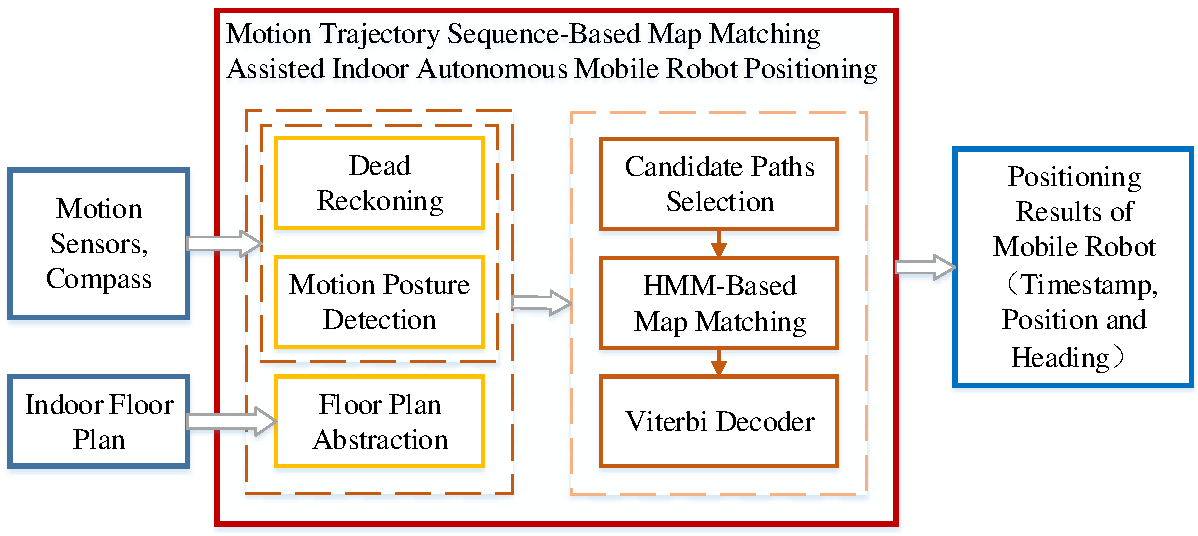
\includegraphics[width=4.8in]{RobotMatch-Architecture}
	\caption{System architecture of mobile robot positioning algorithm.}
	\label{fig-architect}
\end{figure}

The overall architecture of mobile robot positioning algorithm presented in this paper is shown in Fig. \ref{fig-architect}. The sensor data and the indoor floor plan are used as the input of the positioning algorithm. The sensor data is collected by the inertial sensors of the mobile robot and the indoor floor plan is obtained by manually input or the indoor electronic map construction algorithm such as SLAM technology. The indoor floor plan abstraction module translates the indoor floor plan into a directed graph, and the dead reckoning module and the motion posture detection module use the sensor data to give the relative displacement and position-related postures of the mobile robot respectively. The goal of map matching module is to match the motion trajectory of the mobile robot with the sequence of nodes in the directed graph, and then estimate the real time position of the mobile robot. First, the road segments are selected according to the heading direction estimation and the connection of road segments. Secondly, this algorithm updates the related parameters in the hidden Markov model according to the latest candidate road segments. Finally, it estimates the possibilities of all the alternative roads through the Viterbi decoder. When the proposed algorithm is in the convergence stage, the most possible alternative road is the optimal estimation. The final output of the algorithm proposed in this paper is the real-time position and heading direction of mobile robot.

\subsection{Indoor Floor Plan Abstraction}

The posture-related positions divide the indoor roads into road segments. Taking the road segment as a node, the posture change pattern from one road segment to another as a directed edge, the indoor floor plan can be abstracted as a directed graph. Fig. \ref{fig-abstract} shows an example of indoor floor plan and its corresponding directed graph. In this paper, a node is represented by the tuple $(id,{x_1},{y_1},{x_2},{y_2},{\varphi _1},{\varphi _2})$, where ${x_i},{y_i},i = 1,2$ represent coordinates of the two endpoints of the road segment, ${\varphi _1},{\varphi _2}$ represent the heading direction when the mobile robot moves on the road segment and reaches the corresponding endpoint. A tuple $(i{d_1},i{d_2},x,y,change\ of\ motion\ attitude(MA))$ represents a directed edge between nodes, where, $i{d_1}$ denotes the identity of the starting node, $i{d_2}$ denotes the identity of the end node and $x,y,$\emph{MA} represent the coordiantes of position and the change of motion attitude from the starting node to the end node, respectively.

\begin{figure}[!htbp]
	\centering
	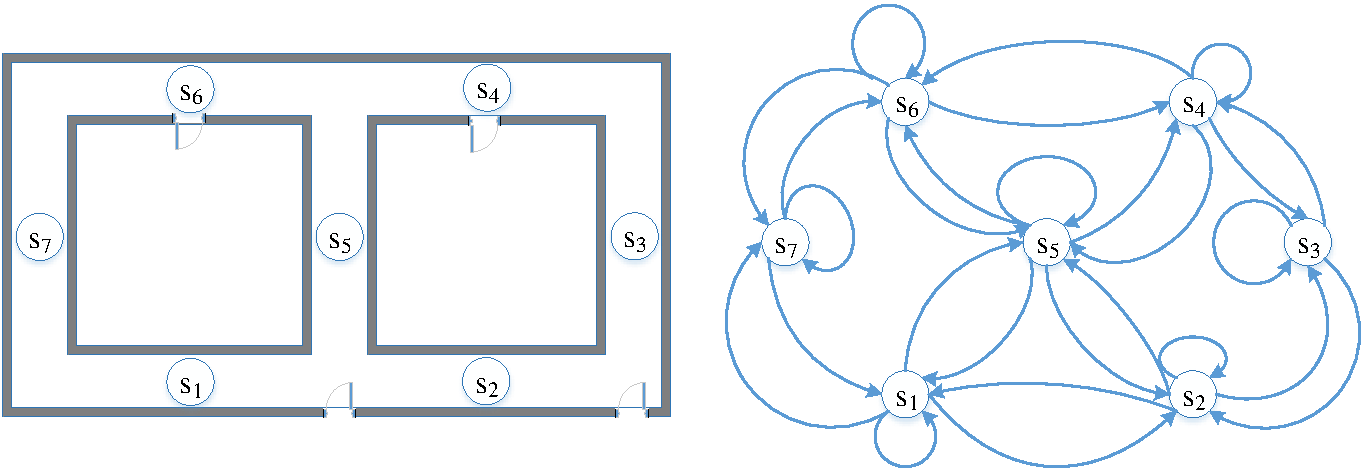
\includegraphics[width=4.576in]{RobotMatch-MapAbstract}
	\caption{Indoor floor plan example and its corresponding directed graph.}
	\label{fig-abstract}
\end{figure}

\subsection{Motion Posture Detection}

This section presents a decision tree model for the motion posture detection of indoor mobile robots. This paper focuses on the positioning of mobile robots in indoor 2D plane. Therefore, our decision tree considers only the relevant postures detection of a mobile robot on the plane, including stationary, go straight, left/right turns and U-turns.

The horizontal movement posture of the indoor autonomous mobile robot is distinguished by different modes of the horizontal component of the accelerometer and the vertical component of the gyroscope in the mobile robot, where the horizontal component of the accelerometer is the data of $Y$-axis in the local coordinate system of the mobile robot and the vertical component of the gyroscope is the data of $Z$-axis in the robot's local coordinate system. Furthermore, by extracting the vertical component of the accelerometer, this method can be easily extended to three-dimensional indoor positioning scenes.

\begin{figure}[!htbp]
	\centering
	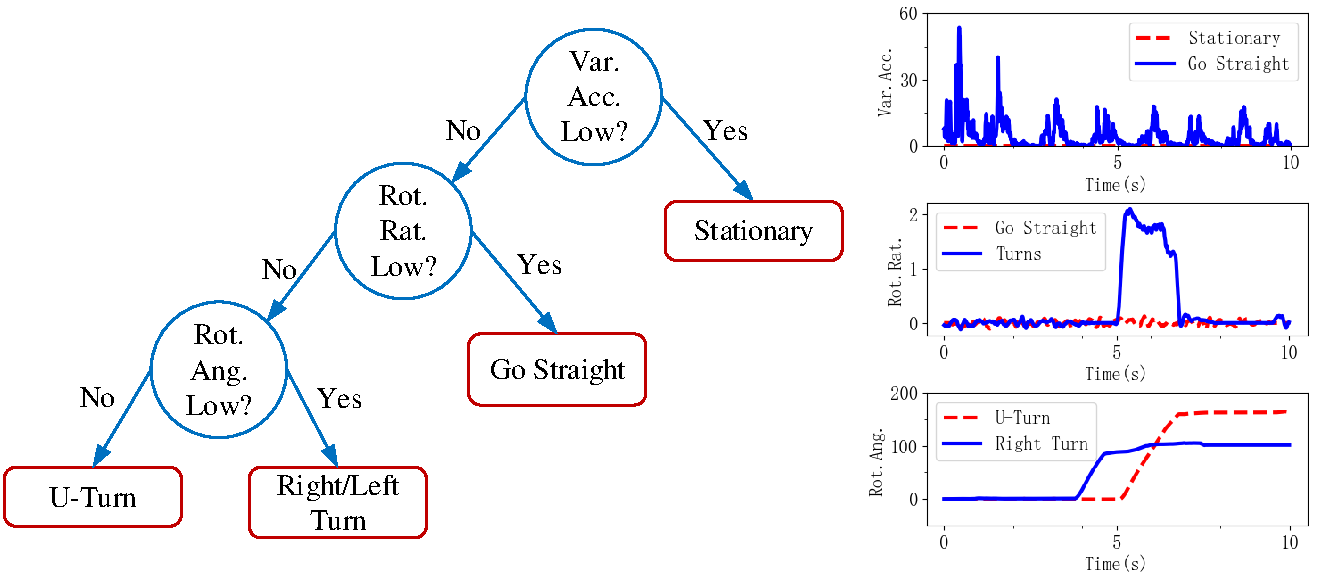
\includegraphics[width=4.95in]{RobotMatch-ActivityDecision}
	\caption{Decision tree for motion posture detection.}
	\label{fig-posture}
\end{figure}

Fig. \ref{fig-posture} shows a decision tree for the motion posture detection of an indoor autonomous mobile robot. The decision tree uses the signal characteristics of built-in acceleration and gyroscope to identify different motion posture patterns of the mobile robot. Considering that the linear velocity of the mobile robot is obtained from the integration of the acceleration horizontal component in time, the instantaneous velocity has an accumulated error at a certain moment. Therefore, the top layer of the decision tree uses the variance of the acceleration horizontal component to separate the stationary and going straight; the second level of the decision tree uses the rotation rate measured on the $Z$-axis of the gyroscope to separate turns and going straight; finally, the third level of the decision tree uses the rotation angle to separate the U-turn from the left or right turn.

\begin{table}
	\label{table_conf}
	\caption{Confusion Matrix of Motion Posture Detection}
	\begin{center}
		\begin{tabular}{| c || c | c | c | c |}
			\hline
			\bfseries Motion Posture & \bfseries Left Turn & \bfseries Right Turn & \bfseries U-turn & \bfseries Go Straight\\
			\hline\hline
			\bfseries Left Turn & 58 & 0 & 2 & 0 \\
			\hline
			\bfseries Right Turn & 0 & 58 & 1 & 1 \\
			\hline
			\bfseries U-turn & 0 & 0 & 60 & 0 \\
			\hline
			\bfseries Go Straight & 0 & 0 & 0 & 60 \\
			\hline
		\end{tabular}
	\end{center}
\end{table}

In the real experimental environment, the four-wheeled differential-driving robot described in the Section $2.1$ is used to finish left-turning, right-turning, U-turn, and straight-motion. Each sample is sampled for $4$ seconds and the valid sample number of each motion posture is $60$. The classification results obtained by the above decision tree model are shown in Table $1$.

\section{HMM based Map Matching Algorithm}

With the help of the motion posture detection based on inertial sensor data, the motion trajectory of the mobile robot can be divided into sub-trajectory segments by position-related postures, such as left or right turn and U-turn, and these sub-trajectory segments form a sub-trajectory sequence in the time dimension. This section gives a detailed description of Hidden Markov Models for matching sub-trajectory sequence to indoor abstract graph.

\subsection{Hidden Markov Model}

A Hidden Markov Model is a time-series probability model that describes the state of a process using discrete random variables. A basic HMM can be represented as $\lambda  = (S,V,A,B,\pi)$, where:

1) $S = \left\{ {{s_1},{s_2},{s_3}, \ldots ,{s_N}} \right\}$ is the set of possible hidden states and $N = \left| S \right|$. In our case, each state represents an indoor road segment, that is, a node of the directed graph. Therefore, a state $s$ is represented by the tuple in the form of ($id,x_{1},y_{1},{\varphi}_{1},x_{2},y_{2},{\varphi}_{2}$), where $id$ is the identification of road segment, $x_{1}$, $y_{1}$, ${\varphi}_{1}$, $x_{2}$, $y_{2}$ and ${\varphi}_{2}$ are different attributes of node of the directed graph, respectively. It should be noted that if the mobile robot can reach another road segment by going straight from one road segment, these two road segments can be merged into a new road segment, also a new hidden state. The road segments $s_4$, $s_6$ can be combined into new road segments as shown in Fig. \ref{fig-viterbi}.

2) $V = \left\{ {{v_1},{v_2},{v_3}, \ldots ,{v_M}} \right\}$ is the set of observations from the model and $M = \left| V \right|$. In our case, an observable state represents the relative movement distance and heading direction measured by motion sensors installed in the mobile robot and is represented in terms of $(dist,\varphi)$.

3) $A = \left\{ {{a_{ij}}} \right\}$ is the state transition probability distribution, where \\ ${a_{ij}} = p\left\{ {{q_{t + 1}} = {s_j}|{q_t} = {s_i}} \right\}, i, j \le N$, where ${q_t}$ denotes the state at time $t$. In other words, $a_{ij}$ indicates the possibility of moving from one road segment to adjacent road segments.

4) $B = \left\{ {{b_i}(k)} \right\}$ is the observation probability distribution in state $i$, where ${b_i}(k) = p\{ {z_t} = {v_k}|{q_t} = {s_i}\},1 \le i \le N,1 \le k \le M$ and $z_t$, $q_t$ are the observation and state at time $t$, respectively. In other words, ${b_i}(k)$ indicates the possibility of a certain distance and heading direction measured by the inertial sensors after the mobile robot has passed a road segment.

5) $\pi  = \left\{ {{\pi _i}} \right\}$ is the initial state distribution, where ${\pi _i} = p\left\{ {{q_1} = {S_i}} \right\},1 \le i \le N$.

\subsection{Transition Probability Distribution (A)}

The transition probability distribution refers to the possibility of moving from a hidden state to the next hidden state. In this paper, it also means the possibility of moving from one road segment to the adjacent road segment. The adjacent road segments are divided by posture-related positions. Each posture-related position has a corresponding motion posture. The higher the degree of matching between the mobile robot's motion posture and position-related posture is, the greater the probability that the mobile robot moves from one road segment to another road segment through this posture-related position is, and vice versa. Therefore, we use the degree of matching between the motion posture of the mobile robot and position-related posture to represent the transition probabilities between adjacent road segments. Let $e^{ij}$ denote the edge of the directed graph from $s_i$ to $s_j$, the corresponding position-related posture can be represented by $e^{ij}$.MA according to definition in Section $2.3$. Given the motion posture of the mobile robot $Rob_{MA}(t)$ at time $t$. The probability from $s_i$ to $s_j$ is shown in Equation \ref{equ-transition}, where $p(Ro{b_{MA}}(t)|{e^{ij}}.MA)$ can be obtained from the motion posture confusion matrix in Section $2.4$.
\begin{equation}
     \label{equ-transition}
	p({s_{j,t}}|{s_{i,t - 1}}) = p({s_j}|{s_i},Ro{b_{MA}}(t)) = p(Ro{b_{MA}}(t)|{e^{ij}}.MA)
\end{equation}

\subsection{Observation Probability Distribution (B)}

In this paper, an observable state consists of the relative displacement of the mobile robot and the heading direction, and the two are independent of each other. Therefore, the observable probability distribution can be defined as:

\begin{equation}
	P({v_{k,t}}|{s_{j,t}}) = P(\varphi (t)|{s_{j,t}}) \cdot P(dist(t)|{s_{j,t}})
\end{equation}

where, $P(\varphi (t)|{s_{j,t}})$ represents the observable probability of the mobile robot's heading direction at time $t$, and $P(dist(t)|{s_{j,t}})$ denotes the observable probability determined by the relative displacement of the mobile robot.

The higher the degree of matching between the heading direction of the mobile robot and the road segment, the greater the possibility that the mobile robot is located in the road segment. In the indoor environment, the error of the heading direction of the mobile robot not only comes from the accumulation error, but also comes from the interference of various metal materials in the buildings. In general, the error of the heading direction is relatively large and it is difficult to accurately model this error. Therefore, in this paper, Equation \ref{equ-heading} is used to model the heading direction in the observable state.

\begin{equation}
\label{equ-heading}
\begin{array}{l}
P(\varphi (t)|{s_{j,t}})\\
= P\{ \varphi (t)|{s_j}.{\varphi _i},i = 1,2\}  = \left\{ {\begin{array}{*{20}{l}}
	{1,if|\varphi (t) - {s_j}.{\varphi _i}| < {H_{TH}},i = 1,2}\\
	{0,others}
	\end{array}} \right.
\end{array}
\end{equation}

where, $H_{TH}$ is a constant threshold used to determine whether the heading direction of the mobile robot matches the direction of the road segment or not. In order to avoid that the correct road segment is excluded due to the large error of the heading direction, $H_{TH}$ is set to $59{\rm{^\circ }}$ in this paper.

The relative displacement error of the mobile robot mainly comes from the accumulative error caused by the acceleration error in the dead reckoning process. Here we assume that the relative displacement of the mobile robot obeys the Gaussian distribution. On the one hand, intuitively speaking, the closer the relative displacement of the mobile robot and the length of the road segment is, the more likely the mobile robot is located in the road segment; on the other hand, For the road segments whose lengths are much larger than the relative displacement of the mobile robot, all of them should have the same possibility. Combining the above two situations, this paper uses Equation \ref{equ-obv-dist} to model the relative displacement in the observable state.

\begin{equation}
\label{equ-obv-dist}
\begin{array}{l}
P(dist(t)|{s_{j,t}})\\
= P\{ dist(t)|{s_j}.dist\}  = \left\{ {\begin{array}{*{20}{l}}
	{\frac{1}{{\sqrt {2\pi } {\sigma _d}}}{e^{ - 4.5}},dist(t) + 3{\sigma _d} \le {s_j}.dist}\\
	{\frac{1}{{\sqrt {2\pi } {\sigma _d}}}{e^{ - \frac{{{{(dist(t) - {s_j}.dist)}^2}}}{{2{\sigma _d}^2}}}},others}
	\end{array}} \right.
\end{array}
\end{equation}

Where ${s_j}.dist$ is the length of the road segment, which can be derived from the two endpoints of the road segment $s_j$ and $\sigma _d$ is the standard deviation of the relative displacement of the mobile robot at time $t$. In order to estimate the value of $\sigma _d$, this paper firstly tests the change of the accelerometer's value $\Delta a$ when the mobile robot is stationary, and estimates the standard deviation of the acceleration $\sigma_a$ based on the absolute median error (MAD) of the test data \cite{aly2015semmatch}. It can be inferred that there is a secondary relationship between $\sigma _d$ and $\sigma _a$ according to the principle of the dead reckoning described in Section $2.1$.

\begin{equation}
	{\sigma _a} = 1.4826 \times median(\left| {\Delta a} \right|)
\end{equation}

\subsection{Initial State Distribution}

If the starting point of the mobile robot is already known, then the road segment where the starting point is located is the initial state, and the probability is set to $1$; if the starting point of the moving robot is unknown, all candidates can be selected by Equation \ref{equ-heading} based on the initial heading direction information of the mobile robot and the initial probability distribution is a uniform distribution over the candidate road segments. Correspondingly, the starting point of the mobile robot is assumed to be the average of the starting points of all candidate road segments. In this paper, the initial heading direction of a mobile robot can be obtained from the digital compass or set manually.

\subsection{Optimal Motion Trajectory Estimation}

Based on the above-defined Hidden Markov Model, this paper uses Viterbi algorithm to determine the optimal estimation of the moving trajectory of a mobile robot. For a given observable state sequence $({z_1},{z_2},...,{z_k})$, the goal of the Viterbi algorithm is to find the most possible hidden state sequence $({q_1},{q_2},...,{q_k})$. Fig. \ref{fig-viterbi} briefly illustrates the decoding process of the Viterbi algorithm.

\begin{figure}[!htbp]
	\centering
	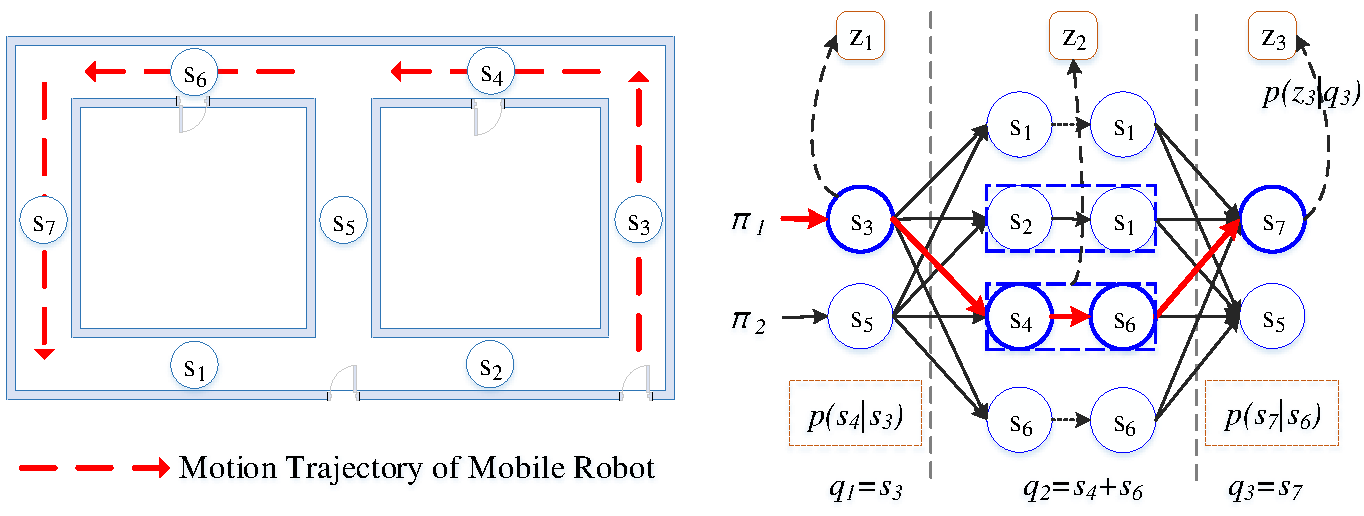
\includegraphics[width=4.976in]{RobotMatch-ViterbiDecoding}
	\caption{Illustration of the proposed HMM model Viterbi decoding.}
	\label{fig-viterbi}
\end{figure}

The Viterbi decoder is implemented by the dynamic programming method. First, a Viterbi variable is defined to represent the maximum probability that the Hidden Markov Model will reach the state $s_i$ along a path at time $t$:

\begin{equation}
	{\delta _t}(i) = \max P\{ {q_1},{q_2}, \cdots ,{q_t} = {s_i},{z_1},{z_2}, \cdots ,{z_t}|\lambda \}
\end{equation}

At time $t$+$1$, the maximum probability reaching the hidden state $s_j$ can be recursively derived from the Viterbi variable at time $t$ by the following equation. 

\begin{equation}
	{\delta _{t + 1}}(j) = [\mathop {\max }\limits_i ({\delta _t}(i) \cdot P\{ {q_{t + 1}} = {s_i}|{q_t} = {s_j}\} )] \cdot P\{ {z_{t + 1}}|{q_{t + 1}}\} ,1 \le t \le k
\end{equation}

By recording the backward pointers, at time $k$, the most likely hidden state sequence, that is, the optimal estimation of the motion trajectory of the mobile robot can be obtained by the path backtracking method. Algorithm $1$ summarizes the processing flow of the trajectory sequence map matching algorithm presented in this paper. 

\begin{algorithm}[H]
	\caption{Motion trajectory sequence-based map matching algorithm}
	\label{alg_aifi}
	\begin{algorithmic}[1]
		
		\renewcommand{\algorithmicrequire}{\textbf{Input:}}
		\renewcommand{\algorithmicensure}{\textbf{Output:}}
		\REQUIRE Sensor data up to current time t: $data_{1:t}$
		\REQUIRE Abstraction of indoor floor plan: $fp$
		\ENSURE Optimal state sequence estimation at current time $t$: $Q_t$
		\ENSURE Mobile robot's position and posture estimation at current time $t$: ${Rob}_t$
		
		\renewcommand{\algorithmicrequire}{\textbf{Define:}}
		\REQUIRE Starting time of current sub-trajectory: $st$, the initial value of $st$ is $0$
		\REQUIRE Length of current motion trajectory sequence: $k$, the initial value of $k$ is $1$
		\REQUIRE Array of Viterbi variables and backward pointers: ${Vtb}_{k}(t)$
		\REQUIRE Candidate road segment list at current time: $S(t)$
		
		
		\STATE ${{Rob}_{t}.{MA}}, at \leftarrow Posture\_Detect({data_{1:t}})$
		
		\IF{${{Rob}_{t}.{MA}}\ != \ None$}  
		
			\STATE ${st} \leftarrow {at}$  
			
			\STATE // Calculate the transition probability TR[ ][ ]
			\FOR{$s_i\ in\ S(t-1)$}
			\STATE $S^i(t) \leftarrow Candidate\_Select(fp, s_i)$
			\FOR{$s_j\ in\ S^i(t)$}
			\STATE TR[i][j] $\leftarrow p(s_j|s_i,Rob_t.MA)$
			\ENDFOR
			\STATE $S(t).extend(S_i(t))$
			\ENDFOR
			
			\STATE // Calculate the observation probability OB[ ]
			\STATE $z(t) \leftarrow Dead\_Reckoning(data_{st:t})$
			\FOR{$s_i\ in\ S(t)$}
			\STATE OB[i] $\leftarrow p(z(t)|s_i)$
			\ENDFOR
			\STATE $Vtb_{k+1}(t) \leftarrow Viterbi\_Calculate(Vtb_{k}(t-1)$, OB[ ], TR[ ][ ]$)$
			\STATE $k$+=1
		
		\ELSE // Not a position-related posture
		
			\STATE // Calculate the observation probability OB[ ]
			\STATE $z(t) \leftarrow Dead\_Reckoning(data_{st:t})$
			\STATE $S(t) \leftarrow S(t-1)$
			\FOR{$s_i\ in\ S(t)$}
			\STATE OB[i] $\leftarrow p(z(t)|s_i)$
			\ENDFOR
			
			\STATE $Vtb_{k}(t) \leftarrow Viterbi\_Calculate(Vtb_{k}(t-1)$, OB[ ]$)$
			
		\ENDIF
		
		\STATE $Q_t \leftarrow Viterbi\_Decoder(Vtb_{k}(t))$
		\STATE $Rob_t \leftarrow Update\_Estimation(data_{st:t}, Q_t)$
		
		\State return $Q_t, Rob_t$
	\end{algorithmic}
\end{algorithm}


\section{Evaluation}

We uses the wheeled mobile robot described in Section $2$ to complete the experimental analysis. The experimental environment is the fifth floor of a teaching hall on our campus. The experimental area is divided into east and west parts, and the east part is approximately $84.85 * 66.8\ (m^2)$. The west part is approximately $68.7 * 106.75\ (m^2)$, the length of connecting corridor between two parts is $46.25\ m$ and the width is $2.4\ m$. The overall layout is shown in Fig. \ref{fig-environment}. In order to record the real position of the robot during the movement, this article divides the experimental area into squares of $0.8 * 0.8\ (m^2)$ and marks every small areas. In the experiment process, another mobile robot with camera is used to move in parallel with the robot to record real-time positions. In the experimental area, the robot moves along the two planned trajectories denoted as $T_1$ and $T_2$ in Fig. \ref{fig-environment}. The length of $T_1$ is $181.9\ m$, including $3$ posture-related positions. The whole trajectory is divided into $4$ sub-trajectories. The length of $T_2$ is $180.5\ m$, including $2$ posture-related positions, the whole trajectory is divided into $3$ sub-trajectories, and the mobile robot repeats $9$ times for each trajectories.

\begin{figure}[!htbp]
	\centering
	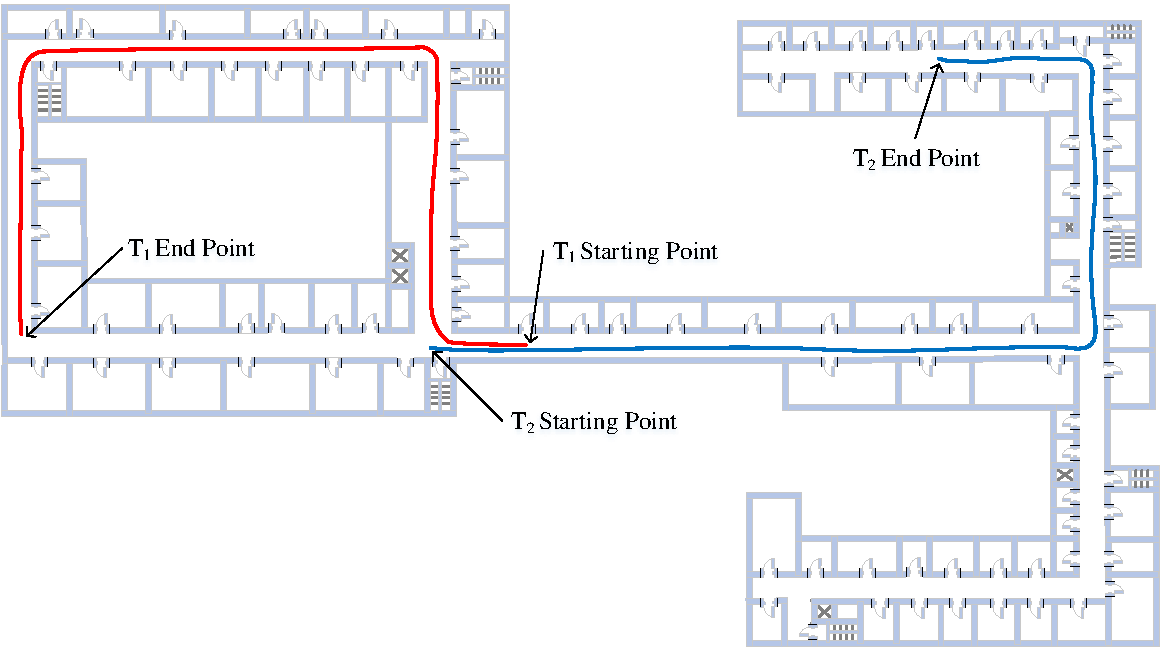
\includegraphics[width=4.976in]{RobotMatch-Environment}
	\caption{Indoor floor plan of experimental environment and mobile robot trajectories.}
	\label{fig-environment}
\end{figure}

\subsection{Influence of Heading Direction Errors}

When the starting point is unknown, the convergence performance of the algorithm is closely related to the detection results of position-related postures. In general, after at least correctly detected two consecutive position-related postures, the map matching algorithm based on the posture detection is likely to converge. Facing the position-related posture detection in 2D floor plan, such as left and right turning, the error of the heading direction has a greater impact on the detection results. Therefore, this section first analyzes the influence of heading direction error on the convergence performance of map matching algorithm. Here, we first define the precision of position-related posture detection by Equation \ref{equ-prec-detect}.

\begin{equation}
\label{equ-prec-detect}
	{Precison} = \frac{Number\ of\ Correctly\ Detected\ Consecutive\ Two\ Postures}{Total\ Number\ of\ Consecutive\ Two\ Postures}
\end{equation}

Supposing that the distribution of the heading direction estimation error obeys Gaussian and the average is $0$. Based on the raw data of the heading direction, a Gaussian random value is added to simulate different degrees of error. Fig. \ref{fig-headingerror} shows the variation of the precision of position-related posture detection under different values of the standard deviation of the heading direction error. It can be seen from Fig. \ref{fig-headingerror} that the precision of position-related posture detection is stable under certain heading direction error conditions, but when the standard deviation of heading direction error reaches a certain level ($T_1$ is $40{\rm{^\circ }}$ and $T_2$ is $30{\rm{^\circ }}$), the precision drops rapidly.

\begin{figure}[!htbp]
	\centering
	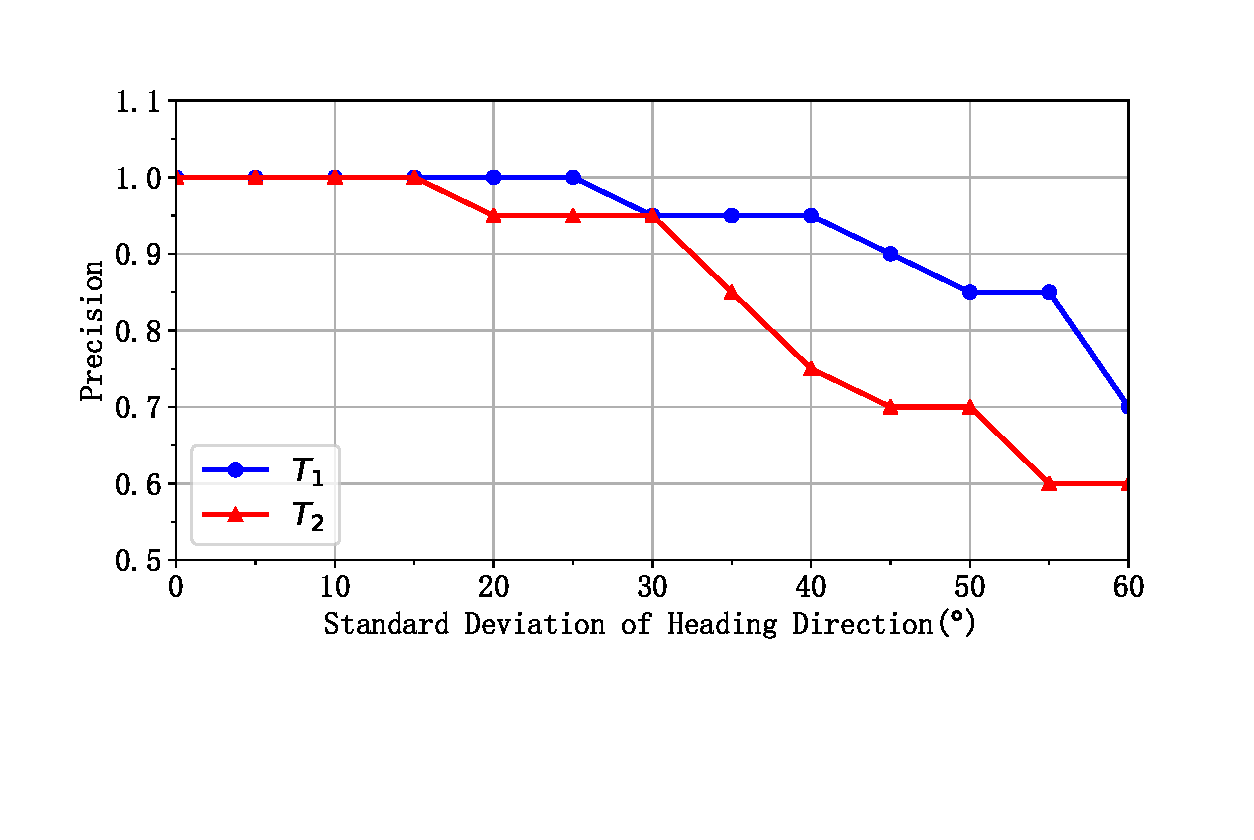
\includegraphics[width=3.976in]{RobotMatch-HeadingError}
	\caption{Heading errors on the precision of mobile robot posture detection.}
	\label{fig-headingerror}
\end{figure}

\subsection{Convergence Speed Analysis without Knowing the Starting Point}

If the starting point is unknown, after the mobile robot moves a certain distance, the algorithm can still converge and finally estimate the real-time position of the mobile robot. The distance before convergence of the algorithm represents the convergence performance of the positioning algorithm. In order to evaluate the convergence performance of the proposed map matching algorithm, we compare the proposed map matching algorithm with the \emph{semMatch} algorithm proposed in \cite{aly2015semmatch} because \emph{semMatch} has certain similarities with the algorithm presented in this paper. The hidden Markov model is also used to implement map matching operations in \emph{semMatch}, however, the details of the HMM model are slightly different.

\begin{figure}[!htbp]
	\centering
	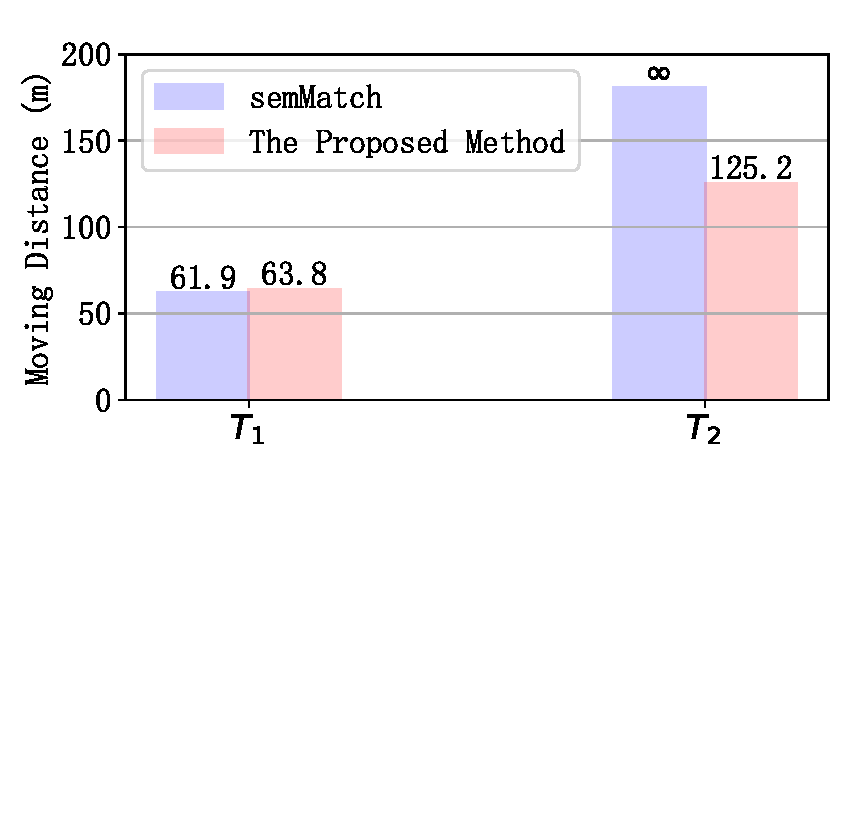
\includegraphics[width=3.276in]{RobotMatch-Convergence}
	\caption{Distance traveled before convergence for each trajectory.}
	\label{fig-convergence}
\end{figure}

Using the same decision tree model to detect the position-related postures in the trajectory of mobile robot, Fig. \ref{fig-convergence} shows the convergence performance of the two algorithms. On the one hand, for $T_1$, both algorithms reach the convergence state after passing through two posture-relate positions. However, the algorithm proposed in this paper needs to observe the subsequent road segment after detect the corresponding posture, so the convergence performance is slightly worse. When it reaches the convergence state, the mobile robot moves $1.9\ m$ more. On the other hand, for $T_2$, the algorithm proposed in this paper reaches the convergence state shortly after the correct detection of the first position-related posture, but \emph{semMatch} does not converge due to the symmetry of indoor road network denoted by $\infty$ in Fig. \ref{fig-convergence}. The main reason is the difference in the HMM model definition of the two map matching algorithms. The hidden state of the map matching algorithm proposed in this paper is the straight road segment in the indoor road network. For $T_2$, the mobile robot firstly pass a long enough road segment, and the proposed algorithm combines this observable state with the subsequent detection of the first position-related posture to achieve the convergence.


\subsection{Online Positioning Performance with Knowing the Starting Point}

If the starting point is already known, the proposed algorithm does not need to pass the motion trajectory matching stage to converge. After convergence, the algorithm can track the moving trajectory of the mobile robot in real time. We use the Euler distance between the real position of the mobile robot and the position estimate given by the algorithm to analyze the real-time positioning performance. Fig. \ref{fig-online} shows the variation of positioning error of the mobile robots with increasing distances on both $T_1$ and $T_2$ trajectories.

\begin{figure}[!htbp]
	\centering
	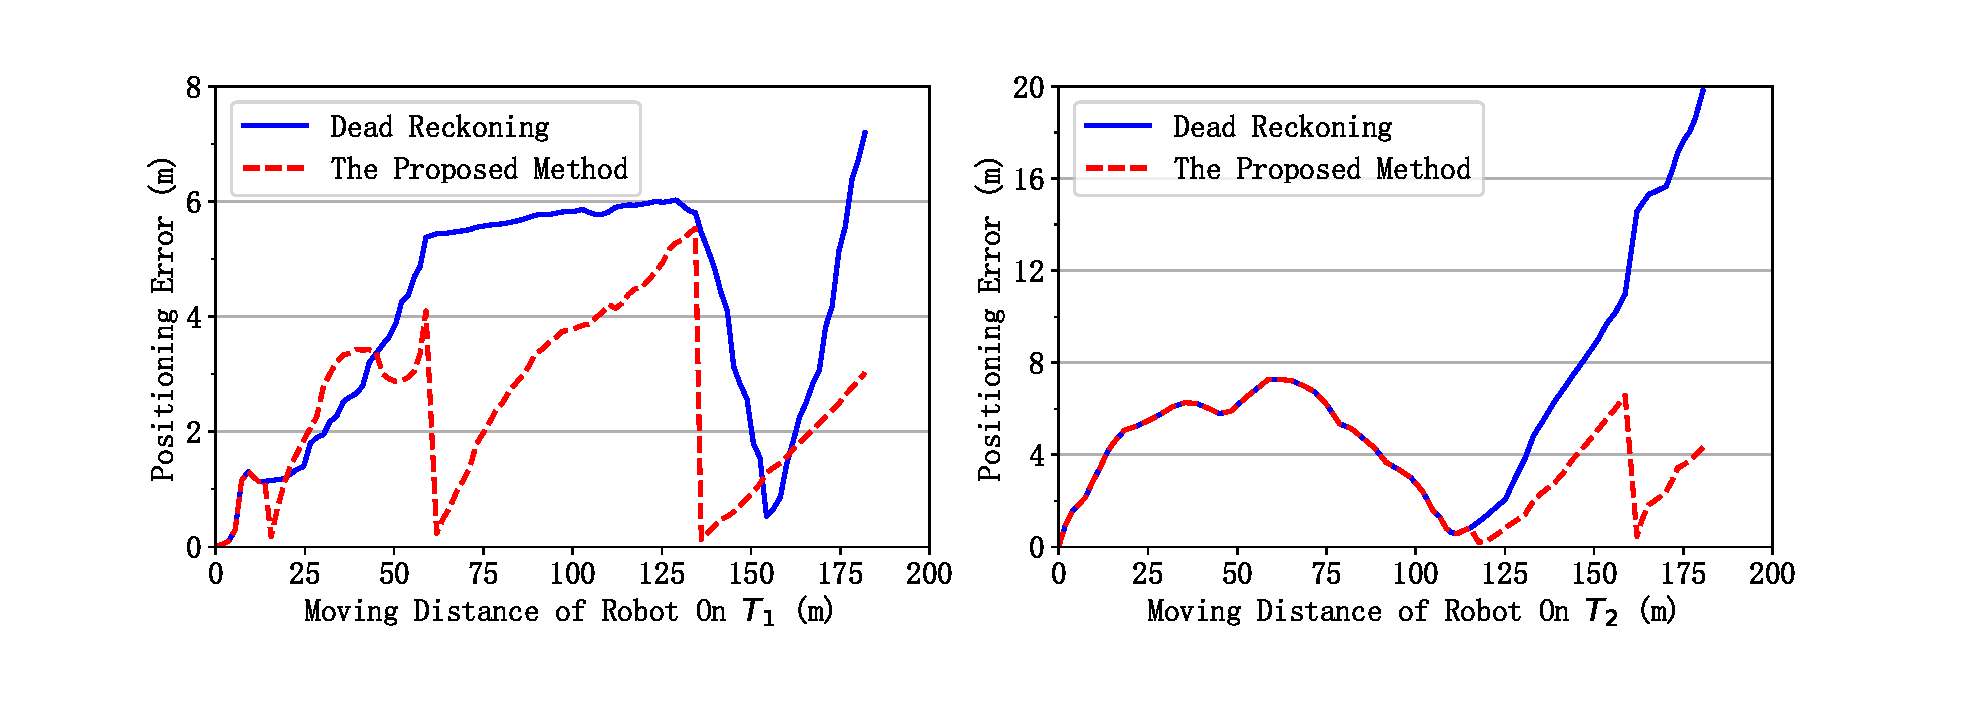
\includegraphics[width=5.076in]{RobotMatch-OnlineError}
	\caption{Online positioning errors for each trajectory.}
	\label{fig-online}
\end{figure}

When the motion trajectory does not include posture-related positions, the map matching assisted positioning technology proposed in this paper is equivalent to the traditional dead reckoning technology, but after detecting the posture-related positions, the known coordinates of the posture-related positions can be used to calibrate the real-time position estimation of the robot. The real-time positioning results of the mobile robot on $T_1$ and $T_2$ shown in Fig. \ref{fig-online} verify this trend. For $T_1$, the average positioning error decreases from $4.0\ m$ to $2.49\ m$, while for $T_2$, the average positioning error decreases from $6.58\ m$ to $3.39\ m$. From the experimental results, it can be deduced that in the actual environment, with the density of posture-related positions increasing, the improvement of positioning performance of the proposed algorithm is more obvious.


\subsection{Influence of Acceleration Errors}

From the principle of dead reckoning technology described in Section $2.1$, we know that the acceleration error has a quadratic relationship with the error of the moving displacement estimation of the mobile robot. Therefore, the acceleration error is one of the main sources of accumulation error in dead reckoning technology. This section simulates different acceleration error degrees by adding Gaussian random values to the raw acceleration data, and then analyzes the influence of the acceleration error on the positioning algorithm proposed in this paper.

\begin{figure}[!htbp]
	\centering
	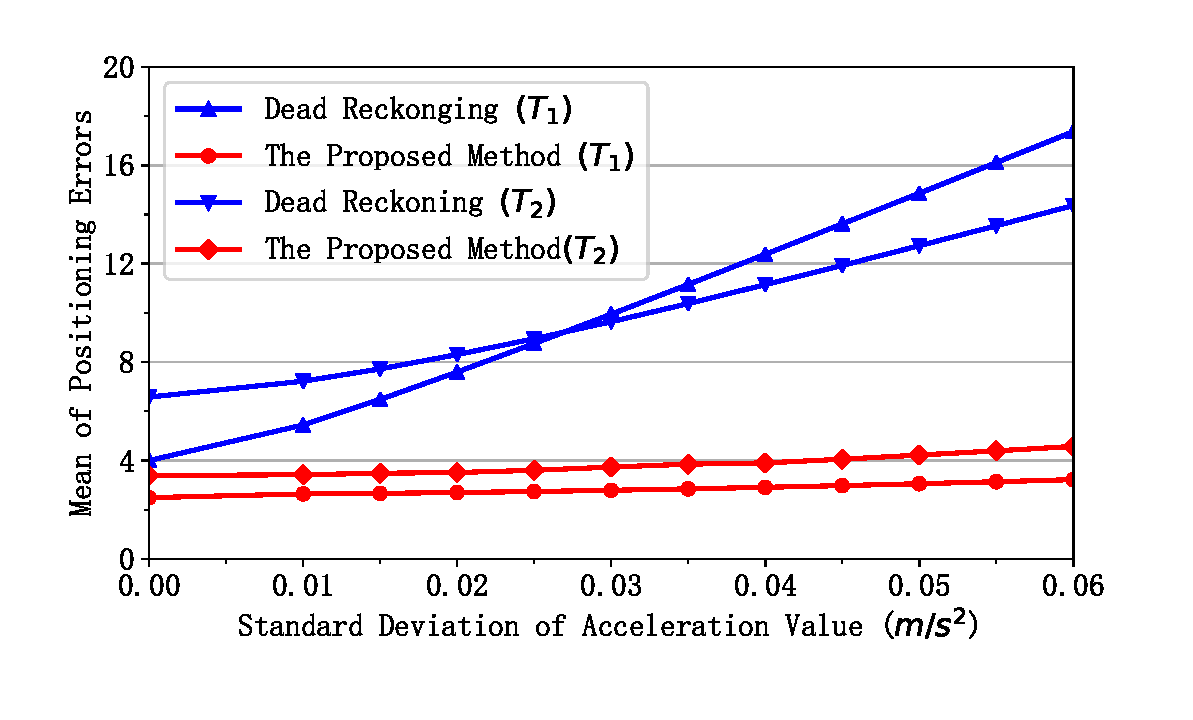
\includegraphics[width=3.676in]{RobotMatch-AcceError}
	\caption{Acceleration value errors on the mean of positioning errors for each trajectory.}
	\label{fig-acce-error}
\end{figure}

Fig. \ref{fig-acce-error} shows the average positioning error of the mobile robots on the two trajectories $T_1$ and $T_2$ under different acceleration error degrees. On the one hand, with a slight increase in the acceleration error, the average of positioning errors rapidly increases, which means that the positioning performance of positioning algorithms based on dead reckoning technology is very sensitive to the acceleration error; on the other hand, with the same variation of acceleration error, compared with the traditional dead reckoning technology, the positioning error of the proposed algorithm changes more smoothly, which shows that the proposed algorithm has a certain degree of robustness to the acceleration error.
 

\section{Conclusion}

In order to solve the difficult problem of positioning of autonomous mobile robots in dark complex building corridors, subway tunnels, or underground mines after sudden accident such as a fire, this paper proposes an indoor autonomous mobile robot tracking and positioning algorithm based on a novel hidden Markov Model. In the structured indoor environment, this method uses the detection of position-related postures to match the motion trajectory of mobile robot to the abstraction of indoor floor plan. Compared with the traditional dead reckoning technology, the proposed algorithm can significantly reduce the influence of cumulative errors on the positioning accuracy, and is robust to the heading direction and acceleration value noises within a certain error range. This algorithm does not rely on cameras, and uses only motion sensors installed in autonomous mobile robots and known indoor floor plan to achieve fusion positioning of dead reckoning and map matching techniques, even when the starting point is unknown. This algorithm has the characteristics of simple deployment, low manufacturing cost and easy operation.

%
% ---- Bibliography ----
%
\bibliographystyle{splncs}
%\bibliographystyle{splncs03_unsrt}
%\bibliographystyle{unsrt}
%% ------ update by springer lncs ----- %%
%\bibliographystyle{splncs04}
\bibliography{RobotMatch}

\end{document}
